\section{Motivating Example}
\label{sec:motivating-example}

In this section, we illustrate how \textsc{MockDetector} finds mock invocations in unit tests. Our tool identifies invocations on variables which have been assigned an object flowing from a mock creation site either using a forward dataflow may-analysis (Soot-based analysis) or by solving specified declarative constraints (Doop-based analysis).

% explain focal methods first.

To motivate our work, consider Listing~\ref{lis:mockCall}, which presents a unit test case from the Maven project. Line~\ref{line:mock} calls \textit{getRequest()}, invoking it on the mock object \texttt{session}. Line~\ref{line:real} then calls \textit{getToolchainsForType()}, which happens to be the focal method whose behaviour is being tested in this test case. At the bytecode level, the two method invocations are indistinguishable with respect to mockness; to our knowledge, current static analysis tools cannot easily tell the difference between the method invocation on a mock object on line~\ref{line:mock} and the method invocation on a real object on line~\ref{line:real}. Given mockness information, an IDE could provide better suggestions. And the uncertainty about mockness would confound a naive static analysis that attempts to identify focal methods. For instance, Ghafari et al~\cite{ghafari15:_autom}'s heuristic would fail on this test, as it returns the last mutator method in the object under test, and the focal method here is an accessor. 

\paragraph{Basic dataflow analysis} The dataflow analysis based \textsc{MockDetector} implementation maintains an abstraction mapping values (local variables or field references) in Soot's Jimple intermediate representation (IR)~\cite{Vallee-Rai:1999:SJB:781995.782008} to \texttt{MockStatus}, which holds three bits monitoring each value's status being a mock, a mock-containing array, and a mock-containing collection, respectively. The declarative version, which we do not explain in this section, maintains relations that track the same bits.

Figure~\ref{fig:mockMethodIllustration} shows how our dataflow analysis works, and Listing~\ref{lis:mockMethodIllustrationIR} shows the Jimple IR of the code in Figure~\ref{fig:mockMethodIllustration}. At the top of the Jimple IR, we begin with an empty abstraction (no mapping for any values, equivalent to all bits false for each value) before line~\ref{line:lis3line3}. For the creation of \texttt{\$r1} on line~\ref{line:lis3line3} and~\ref{line:lis3line4}, since the call to the no-arg \texttt{<init>} constructor is not one of our hardcoded mock APIs, our analysis does not declare \texttt{\$r1} to be a mock object. In practice, our abstraction simply does not create an explicit binding for \texttt{\$r1}, instead leaving the mapping empty as it was prior to line~\ref{line:lis3line3}; but it would be equivalent to create a new \texttt{MockStatus} with all bits false and bind it to \texttt{\$r1}. Thus, we may conclude that the invocation \texttt{object1.foo()} on line 5 in Figure~\ref{fig:mockMethodIllustration} is not known to be a mock invocation. Tying back to our focal methods application, we would not exclude the call to \texttt{foo()} from being a possible focal method.

On the other hand, our imperative analysis sees the mock creation API \texttt{<org.mockito.Mockito: java.lang.Object mock(java.lang.Class)>} on line~\ref{line:lis3line6} and~\ref{line:lis3line7} in the Jimple IR. It thus adds a mapping from local variable \texttt{r2} to a new \texttt{MockStatus} with the mock bit set to true. When the analysis reaches line~\ref{line:lis3line9}, because \texttt{r2} has a mapping in the abstraction with the mock bit being set, \textsc{MockDetector} will deduce that the call on line~\ref{line:lis3line7} is a mock invocation. This implies that the call to method \textit{foo()} on line 11 in Figure~\ref{fig:mockMethodIllustration} cannot be a focal method.

\paragraph{Basic declarative analysis} Again referring to Listing~\ref{lis:mockMethodIllustrationIR}, this time we ask whether the invocation on line~\ref{line:lis3line9} satisfies predicate \texttt{isMockInvocation}, which we define to hold the analysis result---namely, all mock invocation sites in the program. It does, because that line contains a virtual method invocation, and the receiver object \texttt{r2} for the invocation on that line satisfies predicate \texttt{isMockVar}, which holds all mock-containing variables in the program (Listing~\ref{lst:core} will provide more details later). In this case, \texttt{r2} directly satisfies \texttt{isMockVar}, because line~\ref{line:lis3line6} assigns \texttt{r2} the return value from mock source method \texttt{createMock}, and the call to \texttt{createMock} satisfies predicate \texttt{callsMockSource}, which requires that the call destination \texttt{createMock} be enumerated as a constant in our 1-ary relation \texttt{MockSourceMethod}, and that there be a call graph edge between the method invocation at line~\ref{line:lis3line6} and the mock source method.

\paragraph{Extensions: arrays and collections} While we were designing \textsc{MockDetector}, we observed several cases where developers store mock objects in arrays and collections. Listing~\ref{lis:container} presents method \textit{setUp()} in class \texttt{NodeListIteratorTest} from commons-collections-4.4, where line \ref{line:storeMocksInArray} puts the mock \texttt{Node} objects in the array-typed field \texttt{nodes}. This field is later used in test cases. When the flow function of the dataflow analysis encounters an assignment statement containing an array read or write, it first looks for values (local variables or field reference sources) on the opposite side of the assignment statement---the statement's destination or source, respectively---in the Jimple intermediate representation. It then checks whether any of these local variables or field references have been marked as mock objects in the analysis. If so, then the tool would mark the local variable or field reference representing the array as an array mock---it propagates the mockness to the array container.

Figure~\ref{fig:arrayMockIllustration} illustrates the process of identifying a mock-containing array, and Listing~\ref{lis:arrayIllustrationIR} displays the Jimple IR of the code in Figure~\ref{fig:arrayMockIllustration}. Our analysis reaches the mock API call on line~\ref{line:lis4line4}--\ref{line:lis4line6}, where it records that \texttt{\$r2} is a mock object---it creates a MockStatus abstraction object with mock bit set to 1 and associates that object with \texttt{\$r2}. The tool would then handle the cast expression assigning to \texttt{r1} on line~\ref{line:lis4line7}, giving it the same MockStatus as \texttt{\$r2}. When the analysis reaches line~\ref{line:lis4line9}, it finds an array reference on the left hand side, along with \texttt{r1} stored in the array on the right hand side of the assignment statement. At that point, it has a MockStatus associated with \texttt{r1}, with the mock bit turned on. It can now deduce that \texttt{\$r3} at the left hand is an array container which may hold a mock object. Therefore, \textsc{MockDetector}'s imperative static analysis associates \texttt{\$r3} with a MockStatus with mock-containing array bit (named arrayMock flag) set to 1.

The declarative analysis uses analogous reasoning, but uses a relation \texttt{isArrayLocalThatContainsMocks} instead of a bit in the MockStatus abstraction object.

\begin{lstlisting}[basicstyle=\ttfamily, caption={This code snippet illustrates an example from maven-core, where calls to both the focal method \texttt{getToolchainsForType()} and to mock \texttt{session}'s \texttt{getRequest()} method occur in test \textit{testMisconfiguredToolchain()}.},
basicstyle=\scriptsize\ttfamily,language = Java, framesep=4.5mm, escapechar=|,
framexleftmargin=1.0mm, captionpos=b, label=lis:mockCall, morekeywords={@Test}]
@Test
public void testMisconfiguredToolchain()
                 throws Exception {
    MavenSession session = mock( MavenSession.class );
    MavenExecutionRequest req = 
      new DefaultMavenExecutionRequest();
    when( session.getRequest() ).thenReturn( req ); |\label{line:mock}|
    
    ToolchainPrivate[] basics =
      toolchainManager.getToolchainsForType("basic", session); |\label{line:real}|
    
    assertEquals( 0, basics.length );
}
\end{lstlisting}

\begin{lstlisting}[basicstyle=\ttfamily, caption={This example illustrates a field array container holding mock objects from \textit{setup()} in \texttt{NodeListIteratorTest.java}.},
basicstyle=\scriptsize\ttfamily,language = Java, framesep=4.5mm, framexleftmargin=1.0mm, captionpos=b, label=lis:container, escapechar=|, morekeywords={@Test}]
// Node array to be filled with mock Node instances
private Node[] nodes;
@Test
protected void setUp() throws Exception {
    // create mock Node Instances and 
    // fill Node[] to be used by test cases
    final Node node1 = createMock(Element.class);
    final Node node2 = createMock(Element.class);
    final Node node3 = createMock(Text.class);
    final Node node4 = createMock(Element.class);
    nodes = new Node[] {node1, node2, node3, node4}; |\label{line:storeMocksInArray}|
    // ...
}
\end{lstlisting}


\begin{figure}
\begin{lstlisting}[basicstyle=\ttfamily,
basicstyle=\scriptsize\ttfamily,language = Java, framesep=4.5mm, framexleftmargin=1.0mm, captionpos=b, escapechar=|, morekeywords={@Test}]
//        mock: |\xmark~\,|    mockAPI: |\xmark|
Object object1 = new Object();

// mock: |\xmark|
object1.foo();

//        mock: |\cmark|     mockAPI: |\cmark|
Object object2 = mock(Object.class);

// mock: |\cmark|
object2.foo();
\end{lstlisting}
%    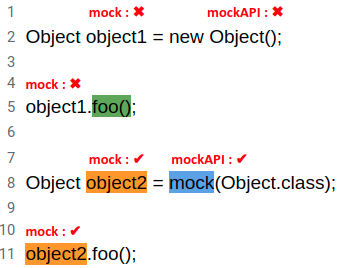
\includegraphics[width=.25\textwidth]{Images/mockInvocationIllustration.png}
    
    \caption{Our static analysis propagates mockness from sources (e.g. \texttt{mock(Object.class}) to invocations.}
    \label{fig:mockMethodIllustration}
    
\end{figure}

\begin{figure}
\begin{lstlisting}[
basicstyle=\scriptsize\ttfamily,language = Java, framesep=4.5mm, framexleftmargin=1.0mm, captionpos=b, escapechar=|, morekeywords={@Test}]
//        mock: |\cmark|     mockAPI: |\cmark|
Object object1 = createMock(Object.class);

// arrayMock: |\cmark| |$\Leftarrow$| array-write    |~~|  mock: |\cmark|
objects  |~~|           = new Object[]  |~|  { object1 };
\end{lstlisting}
    
    \caption{Our static analysis also finds array mocks.}
    \label{fig:arrayMockIllustration}
    
\end{figure}

\begin{lstlisting}[basicstyle=\ttfamily, caption={Jimple Intermediate Representation for the code in Figure~\ref{fig:mockMethodIllustration}.},
basicstyle=\scriptsize\ttfamily, captionpos=b, label=lis:mockMethodIllustrationIR, escapechar=|, morekeywords={@Test, specialinvoke, virtualinvoke, staticinvoke}]
java.lang.Object $r1, r2;

$r1 = new java.lang.Object; |\label{line:lis3line3}|
specialinvoke $r1.<java.lang.Object: void <init>()>(); |\label{line:lis3line4}|
virtualinvoke $r1.<java.lang.Object: void foo()>(); |\label{line:lis3line5}|
r2 = staticinvoke <org.mockito.Mockito: |\label{line:lis3line6}|
        java.lang.Object mock(java.lang.Class)> |\label{line:lis3line7}|
     (class "Ljava/lang/Object;");
virtualinvoke r2.<java.lang.Object: void foo()>(); |\label{line:lis3line9}|
\end{lstlisting}

\begin{lstlisting}[basicstyle=\ttfamily, caption={Jimple Intermediate Representation for the array in Figure~\ref{fig:arrayMockIllustration}.},
basicstyle=\scriptsize\ttfamily, framesep=4.5mm, framexleftmargin=1.0mm, captionpos=b, label=lis:arrayIllustrationIR, escapechar=|, morekeywords={@Test, specialinvoke, virtualinvoke, staticinvoke, newarray}]
java.lang.Object r1, $r2;
java.lang.Object[] $r3;

$r2 = staticinvoke <org.easymock.EasyMock: |\label{line:lis4line4}|
         java.lang.Object createMock(java.lang.Class)>
     (class "java.lang.Object;"); |\label{line:lis4line6}|
r1 = (java.lang.Object) $r2; |\label{line:lis4line7}|
$r3 = newarray (java.lang.Object)[1]; |\label{line:lis4line8}|
$r3[0] = r1;  |\label{line:lis4line9}|
\end{lstlisting}
